%RL->MDP, Q, SARSA, SMDP, 
%MDP
%Model-based
%dynamic programming
%Dyna
%Model-free
%Q
%SARSA
\chapter{Background}
\label{ch:RL}

In this chapter, we introduce the basic concept of reinforcement learning (RL)
and the Markov decision process (MDP) and Semi-Markov decision process (SMDP) formalisms.
We describe the solution methods of MDPs and SMDPs, that include model-free and model-based 
methods. Then we review the concepts and algorithms in hierarchical reinforcement learning (HRL) frameworks. 
We present the brief introduction of previous work in the RL field.
For more comprehensive introduction of MDP, SMDP and RL, please refer to standard text
\cite{howard1960, Puterman94, SuttonIntro, KevinIntro}.
Bertsekas and Tsitsiklis \cite{Neurodynamic} introduce RL from a more theoretic perspective.
A more detailed introduction of HRL can be found in \cite{HRLSurvey}.

\section{Reinforcement Learning}
Reinforcement learning (RL) addresses the problem for an agent to execute a sequence of actions
in a stochastic environment to maximize its rewards. 

In the RL setting, the environment can be modeled in several formalisms.
One of the most commonly adopted formalisms is Markov decision processes (MDPs).
An MDP assumes that the state of the environment is fully observable, and each action takes a single
step to finish. Semi-Markov decision processes (SMDPs) remove the latter assumption and allow
the action to take several time steps. Partially observable Markov decision processes (POMDPs) remove
the former assumption and the agent needs to decide the actions without access to the full state
of the environment.

Regardless of the underlying models of the environment, the objective of an RL method is
to find an optimal policy for the model. MDPs and SMDPs are introduced in Sections \ref{se:MDP} and \ref{se:SMDP}.
POMDPs are orthogonal to our work, thus they will not be covered.
%the MDP is unknown to the agent in the beginning. 
%The task of reinforcement learning
%consists of nding an optimal policy for the associated MDP. We will therefore
%refer to the underlying MDP as the model of the environment (or simply model
%if it is clear from the context which meaning of model is intended). The optimal
%policy is denoted by  and the corresponding utility function by V .

%The lack of an apriori known model generates a need to sample the MDP to
%gather statistical knowledge about this unknown model. Depending on the kind
%of knowledge that is gathered, a distinction is made between model-based and
%model-free solution techniques.

In the RL setting, the environment is modeled as an MDP problem.
However, the MDP is unknown to the RL agent. The objective of reinforcement learning is to 
learn an optimal policy for the MDP. Since the MDP is unknown in the beginning, 
the agent needs to sample the MDP to acquire the knowledge about the MDP.
The learning agent will take actions based on the current state. For the first step, the agent does not know anything about 
the environment, therefore the agent has to choose the first action randomly. After the environment
receives the action, it will provide a reward to the agent as a feedback. The reward can be either
positive or negative. The agent adjusts the value function to maximize the expected reward in the future.
The initial value of value function is 
usually 0, but it is possible to set it to some high enough value to encourage exploration.
It is important to evaluate the value function 
correctly. If some actions with low expected reward are estimated as high, it degrades the
performance of agent.

Reinforcement learning (RL) (Sutton and Barto, 1998) refers to a collection of methods
that allow an agent (a system) to learn how to make good decisions by observing its
own behavior, and improves its actions through a reinforcement mechanism. There are
many formal specifications of this kind of problems that have been developed over the last
fifty years. The most commonly used is the Markov decision processes (MDPs). An
MDP assumes that the agent has full access to the state of the world and each of its actions

%RL methods can be broadly classified into two classes: model-based
%and model-free. Model-based RL learns an effective policy by constructing the model from samples
%and simulating experiences from the model. It generally requires fewer samples to learn the optimal
%policy. However, when the state space is too large, we cannot build the exact model anymore.
%Instead, we have to approximate the model with techniques such as function approximation. Little
%research has been done to address the problem of model-based RL with approximation in an online
%setting.

%TODO: why RL
%TODO: the challenge of RL

%Given a reward function, reinforcement learning algorithms can
%search over possible action space and find a sequence of actions 
%which can maximize the rewards. The reinforcement learning is an ideal choice
%to develop a learning agent for video games.

%In reinforcement learning, the environment can be modeled as an MDP but
%this MDP is unknown to the RL-agent. The task of reinforcement learning
%consists of nding an optimal policy for the associated MDP. We will therefore
%refer to the underlying MDP as the model of the environment (or simply model
%if it is clear from the context which meaning of model is intended). The optimal
%policy is denoted by  and the corresponding utility function by V .

%The lack of an apriori known model generates a need to sample the MDP to
%gather statistical knowledge about this unknown model. Depending on the kind
%of knowledge that is gathered, a distinction is made between model-based and
%model-free solution techniques.



%Reinforcement learning (RL) (Sutton and Barto, 1998) refers to a collection of methods
%that allow an agent (a system) to learn how to make good decisions by observing its
%own behavior, and improves its actions through a reinforcement mechanism. There are
%many formal specifications of this kind of problems that have been developed over the last
%fifty years. The most commonly used is the Markov decision processes (MDPs). An
%MDP assumes that the agent has full access to the state of the world and each of its actions
%takes a single time step. Semi-Markov decision processes (SMDPs) relax the latter
%assumption and allow actions that take several time steps. Finally, partially observable
%Markov decision processes (POMDPs) relax the former assumption by allowing the agent
%to receive observations that do not necessarily reveal the entire state of the environment.
%When a problem is modeled using one of the above, the goal of an RL method is to find a
%good (possibly optimal) policy for the model. We will cover MDPs and SMDPs in detail
%in Sections 2.2 and 2.3. POMDPs will be presented more briefly, as the subject of partial
%observability is almost (but not completely) orthogonal to the main contributions of this
%dissertation.


The agent can select an action which leads to the highest value of value function. However, 
this strategy does not allow the agent to explore the states which are not visited before.
A better approach is to use $\epsilon$-greedy method. The method allows the agent to abandon the
best action and choose
a random action with a very small probability $\epsilon$. The higher the probability, the more
likely that the agent would explore the new actions. However, if the exploration probability 
is too high, it will increase the time to converge.

After the agent takes an action, the environment will provide a reward and a state to the
agent. The agent then decides an new action for the new state. After several iterations
, the agent will learn a correspondence between the action and state. The correspondence is called 
"policy". 

\section{Markov Decision Processes}
\label{se:MDP}
In this work, we address the finite state Markov decision process (MDP) problem:
%\subsection{Model Formulation}
\begin{definition} A Markov decision process is formalized as a tuple $<S, A, P, R, I>$, where:
\begin{itemize}
    \item $S$ is a finite set of states of the environment.
    \item $A$ is a finite set of actions.
    \item $P:S \times A \times S \rightarrow [0, 1]$ is the transition function which defines a probability distribution over the possible next states.
    \item $R:S \times A \times S \rightarrow \mathbb{R}$ is the reward function which defines the reward after executing a certain action at a certain state.
    \item $I:S \rightarrow [0, 1]$ specifies the initial state distribution.
 \end{itemize}
\end{definition}

Given a state of the environment, a policy $\pi: S \rightarrow A$ dictates what action should be performed at that state. 
The Q-function represents the expected cumulative reward after action $a$ is executed in state $s$ and 
policy $\pi$ is followed thereafter.
The value function $V^{\pi}: S \rightarrow \mathbb{R}$ represents the expected cumulative reward when 
policy $\pi$ is followed from state $s$.

The value function satisfies the Bellman equation:
\begin{equation}
    V^{\pi}(s) = \sum_{s'}P(s'|s, \pi(s))[R(s'|s, \pi(s)) + \gamma V^{\pi}(s')],
    \label{eq:V}
\end{equation}
where $\gamma \in [0, 1]$ is the discount factor which discounts the future reward to the present value.

Similarly, we define the action-value function (or Q-function) as:
\begin{equation}
    Q^{\pi}(s, a) = \sum_{s'}P(s'|s, a)[R(s'|s, a) + \gamma Q^{\pi}(s', \pi(s'))].
    \label{eq:Q}
\end{equation}
The Q-function represents the expected cumulative reward after action $a$ is executed at state $s$ and 
policy $\pi$ is followed thereafter.

%\begin{equation}
    %Q^{\pi}(s, a) = \sum_{s', N}P(s', N|s, a)[R(s', N|s, a) + \gamma^N Q^{\pi}(s', \pi(s'))].
    %\label{eq:SMDPQ}
%\end{equation}
%Now lets us extends action set $A$ to include composite actions.

%The transition function $P$ and $R$ are modified to include the time to accomplish each composite action:
%\begin{equation}
    %R(s, a) = \sum^{\infty}_{k=0} \gamma^k r_k
%\end{equation}

%The value function needs to be modified as:
%\begin{equation}
    %V^{\pi}(s) = \sum_{s'}P(s'|s, \pi(s))[R(s, \pi(s), t) + \gamma^N V^{\pi}(s')],
%\end{equation}
%where $N$ is the number of steps for the action $\pi(s)$ to finish its execution.
%A question arises since we do not know the actual time to finish executing each composite action.
%Let's set $gamma=1$ from now on.
%TODO: (how MaxQ solve it?).

%-------------------------------------------------------------------------


\subsection{Solution Method for MDPs}

There are 3 types of reinforcement learning algorithms -- dynamic programming (DP), Monte Carlo 
methods, and temporal-difference (TD). Dynamic programming can compute the optimal policy, but it 
requires a precise model of the environment. In most of the cases, the environment
is too complex to be modeled precisely, and it is not easy to get the complete information about
the environment. On the other hand, it is usually possible to use Monte Carlo method to sample the environment to
get the partial information. 
Like Monte Carlo method, TD uses sampling, therefore it does not require the 
complete model of the environment. TD method is a bootstrapping method, similar to the dynamic 
programming approach, it updates the new value function based on the previous one.

Now that we have defined the MDP model, the next task is to solve it, i.e., to find an
optimal policy and/or the optimal value function.5 There are variety of methods for achieving
this. Some methods require knowing the transition probability and reward functions
and are performed without access to an environment; these are considered offline algorithms.
These are the standard dynamic programming (DP) algorithms from the field of
operations research. Having the model allows the simulation of the domain so as to do
planning to find the optimal value function and/or an optimal policy without interacting
directly with the environment. Other methods work without assuming prior knowledge of
the model and operate by learning through experience in the environment; these are called
online algorithms.
Since a value function (or an action-value function) defines a policy in an MDP, one
approach to find the optimal policy is to compute the optimal value (action-value) function
first, and then extract the optimal policy from it. We call the algorithms utilizing this approach,
value function algorithms. Another approach is to directly find the optimal policy.
The methods using this approach are called policy search methods. In Sections 2.2.4.1 and
2.2.4.2, we present a brief overview of the above two approaches to solve an MDP model.
Value function (VF) methods attempt to find the optimal value (action-value) function
and then extract an optimal policy from it. These algorithms have been extensively studied
1998) and have yielded some remarkable empirical successes in a number of different domains,
including learning to play checkers (Samuel, 1959), backgammon (Tesauro, 1994),
job-shop scheduling (Zhang and Dietterich, 1995), dynamic channel allocation (Singh and
Bertsekas, 1996), and elevator scheduling (Crites and Barto, 1998). We now briefly review
some standard VF algorithms.
If the model is known, then Equation 2.2 defines a system of equations, the solution to
which yields the optimal value function. These equations may either be solved directly via
solving a related linear program (e.g., Gordon (1999); de Farias (2002)), or by iteratively
performing the update
in the machine learning literature (Bertsekas and Tsitsiklis, 1996; Sutton and Barto,
Other instances of offline VF algorithms are asynchronous value iteration and asynchronous
policy iteration (Bertsekas and Tsitsiklis, 1996; Sutton and Barto, 1998).
If the agent does not know the model of the domain, we may first try to interact with the
environment to learn a model which is then used to compute optimal policies (e.g., Dyna
(Sutton, 1991) and prioritized sweeping (Moore and Atkeson, 1993)). This is known as
Model-based approach. Alternatively, we may try to learn the value (action-value) function
directly and do not explicitly learn a model. This approach is referred to as model-free,
in that the agent does not need to learn the transition probabilities. Most of the modelfree
VF algorithms are instances of the temporal difference (TD) learning (Sutton, 1988),
where the agent updates estimates of the value (action-value) function based in part on
other estimates, without waiting for the true value. Two more popular TD methods are
SARSA (Rummery and Niranjan, 1994) and Q-learning (Watkins, 1989).


%\subsubsection{Model-Free Methods}

The equation to compute the value function in TD:
\begin{displaymath}
   V(S_t) \leftarrow V(S_t) + \alpha [r_{t+1} + \gamma V(S_{t+1}) - V(S_t)],
\end{displaymath}

where $V(s_t)$ is the value function of the state $s_t$. $V(s_t)$ is the expected reward when
the agent reaches the state $s_t$. $r_{t+1}$ is the reward given to the agent when it chooses
the action at state $s_t$.

%\section{Q-Learning}
\label{sec:Q-Learning}
    Q-Learning is an off-policy TD approach. Compared to SARSA, Q-Learning updates
the Q value by the highest value of the next possible state-action, rather than the 
next state-action executed by the agent.  
The Q value is updated by:
\begin{displaymath}
   Q(s_t, a_t) \leftarrow Q(s_t, a_t) + \alpha [r_{t+1}+\gamma \max_a Q(s_{t+1},a)-Q(s_t,a_t)],
\end{displaymath}

where $\max_a Q(s_{t+1},a)$ is the highest value of the next possible state-action. 

\begin{center}
\begin{tabular}{@{}lp{6cm}@{}}
\hline
Algorithm: Q-Learning\\
\hline
Initialize $Q(s, a)$ arbitrarily\\
Repeat (for each episode):\\
\ \ \ \ \ \ Initialize $s$\\
\ \ \ \ \ \ Repeat (for each step of episode):\\
\ \ \ \ \ \ \ \ \ \ \ \ Choose $a$ based on $s$ using policy derived from $Q$ (e.g., $\epsilon$-greedy method)\\
\ \ \ \ \ \ \ \ \ \ \ \ Take action $a$, obtain reward $r$ and next state $s'$ from the environment\\
\ \ \ \ \ \ \ \ \ \ \ \ $Q(s, a) \leftarrow Q(s, a) + \alpha [r + \gamma max_{a'} Q(s', a')-Q(s, a)]$\\
\ \ \ \ \ \ \ \ \ \ \ \ $s \leftarrow s'$\\
\ \ \ \ \ \ Until $s$ is terminal\\
\hline  
\end{tabular}
\end{center}

%\section{SARSA}
\label{sec:SARSA}
SARSA is a on-policy TD approach. On-policy indicates that it learns from the current policy.
Different from other TD approaches, SARSA updates the Q value of the current state-action from the next state-action.
The Q value is updated by:
\begin{displaymath}
    Q(s_t, a_t) \leftarrow Q(s_t, a_t) + \alpha [r_{t+1} + \gamma Q(s_{t+1}, a_{t+1})-Q(s_t, a_t)],
\end{displaymath}
where $Q(s, a)$ is the value function for state-pair, and it is the expected reward when the agent takes
the action $a$ at the state $s$. $\alpha$ is step-wise, which controls the learning rate. 
$\gamma$ is the discount factor.


\begin{center}
\begin{tabular}{@{}lp{6cm}@{}}
\hline
Algorithm: SARSA\\
\hline
Initialize $Q(s, a)$ arbitrarily\\
Repeat (for each episode):\\
\ \ \ \ \ \ Initialize $s$\\
\ \ \ \ \ \ Choose $a$ based on $s$ using policy derived from $Q$ (e.g., $\epsilon$-greedy method)\\
\ \ \ \ \ \ Repeat (for each step of episode):\\
\ \ \ \ \ \ \ \ \ \ \ \ Take action $a$, obtain reward $r$ and next state $s'$ from the environment\\
\ \ \ \ \ \ \ \ \ \ \ \ Choose $a'$ based on $s'$ using policy derived from $Q$ (e.g., $\epsilon$-greedy method)\\
\ \ \ \ \ \ \ \ \ \ \ \ $Q(s, a) \leftarrow Q(s, a) + \alpha [r + \gamma Q(s', a')-Q(s, a)]$\\
\ \ \ \ \ \ \ \ \ \ \ \ $s \leftarrow s'$\\
\ \ \ \ \ \ \ \ \ \ \ \ $a \leftarrow a'$\\
\ \ \ \ \ \ Until $s$ is terminal\\
\hline  
\end{tabular}
\end{center}
%\subsubsection{Model-Based Methods}
%\section{Temporal Difference}
%\label{sec:TD}


%\section{}
%SARSA is a on-policy TD approach. On-policy indicates that it learns from the current policy.
%Different from other TD approaches, SARSA updates the Q value of the current state-action from the next state-action.
%The Q value is updated by:
%\begin{displaymath}
    %Q(s_t, a_t) \leftarrow Q(s_t, a_t) + \alpha [r_{t+1} + \gamma Q(s_{t+1}, a_{t+1})-Q(s_t, a_t)],
%\end{displaymath}
%where $Q(s, a)$ is the value function for state-pair, and it is the expected reward when the agent takes
%the action $a$ at the state $s$. $\alpha$ is step-wise, which controls the learning rate. 
%$\gamma$ is the discount factor.

%\begin{center}
%\begin{tabular}{@{}lp{6cm}@{}}
%\hline
%Algorithm: Dyna-Q\\
%\hline
%Initialize $Q(s, a)$ and $Model(s, a)$\\
%Repeat (for each episode):\\
%\ \ \ \ Repeat (for each step of episode):\\
%\ \ \ \ \ \ \ \ $s \leftarrow$ the current state\\
%\ \ \ \ \ \ \ \ Choose $a$ based on $s$ using policy derived from $Q$ (e.g., $\epsilon$-greedy method)\\
%\ \ \ \ \ \ \ \ Take action $a$, obtain reward $r$ and next state $s'$ from the environment\\
%\ \ \ \ \ \ \ \ $Q(s, a) \leftarrow Q(s, a) + \alpha [r + \gamma max_{a'} Q(s', a')-Q(s, a)]$\\
%\ \ \ \ \ \ \ \ $Model(s, a) \leftarrow s', r$
%\ \ \ \ \ \ \ \ Repeat $N$ times:
%\ \ \ \ \ \ \ \ \ \ \ \ $s \leftarrow $ random previously observed state
%\ \ \ \ \ \ \ \ \ \ \ \ $a \leftarrow $ random action previously taken in $s$
%\ \ \ \ \ \ \ \ \ \ \ \ $s', r \leftarrow Model(s, a)$ 
%\ \ \ \ \ \ \ \ \ \ \ \ $Q(s, a) \leftarrow Q(s, a) + \alpha [r + \gamma max_{a'} Q(s', a')-Q(s, a)]$\\
%\hline  
%\end{tabular}
%\end{center}

%\section{The Dyna Architecture}
%SARSA is a on-policy TD approach. On-policy indicates that it learns from the current policy.
%Different from other TD approaches, SARSA updates the Q value of the current state-action from the next state-action.
%The Q value is updated by:
%\begin{displaymath}
    %Q(s_t, a_t) \leftarrow Q(s_t, a_t) + \alpha [r_{t+1} + \gamma Q(s_{t+1}, a_{t+1})-Q(s_t, a_t)],
%\end{displaymath}
%where $Q(s, a)$ is the value function for state-pair, and it is the expected reward when the agent takes
%the action $a$ at the state $s$. $\alpha$ is step-wise, which controls the learning rate. 
%$\gamma$ is the discount factor.

%\begin{center}
%\begin{tabular}{@{}lp{6cm}@{}}
%\hline
%Algorithm: Dyna-Q\\
%\hline
%Initialize $Q(s, a)$ and $Model(s, a)$\\
%Repeat (for each episode):\\
%\ \ \ \ Repeat (for each step of episode):\\
%\ \ \ \ \ \ \ \ $s \leftarrow$ the current state\\
%\ \ \ \ \ \ \ \ Choose $a$ based on $s$ using policy derived from $Q$ (e.g., $\epsilon$-greedy method)\\
%\ \ \ \ \ \ \ \ Take action $a$, obtain reward $r$ and next state $s'$ from the environment\\
%\ \ \ \ \ \ \ \ $Q(s, a) \leftarrow Q(s, a) + \alpha [r + \gamma max_{a'} Q(s', a')-Q(s, a)]$\\
%\ \ \ \ \ \ \ \ $Model(s, a) \leftarrow s', r$
%\ \ \ \ \ \ \ \ Repeat $N$ times:
%\ \ \ \ \ \ \ \ \ \ \ \ $s \leftarrow $ random previously observed state
%\ \ \ \ \ \ \ \ \ \ \ \ $a \leftarrow $ random action previously taken in $s$
%\ \ \ \ \ \ \ \ \ \ \ \ $s', r \leftarrow Model(s, a)$ 
%\ \ \ \ \ \ \ \ \ \ \ \ $Q(s, a) \leftarrow Q(s, a) + \alpha [r + \gamma max_{a'} Q(s', a')-Q(s, a)]$\\
%\hline  
%\end{tabular}
%\end{center}

%--------------------------------

%The lack of an apriori known model generates a need to sample the MDP to
%gather statistical knowledge about this unknown model. Depending on the kind
%of knowledge that is gathered, a distinction is made between model-based and
%model-free solution techniques.
%2.2.1 Model-Based Solution Techniques
%Although the term model-based reinforcement learning is sometimes used to
%refer to solution methods for problems where the MDP is known, we use modelbased
%RL in the traditional sense where methods are considered that do not
%know the model of the world a priori but that do operate by learning this
%model2. This category of approaches is especially important for applications
%where computation is considered to be cheap and real-world experience costly.
%2Another term for these kind of algorithms is indirect reinforcement learning.
%2.2. SOLUTION METHODS 17
%2.2.1.1 Certainty Equivalent Method
%One straightforward method that falls within this category is the certainty
%equivalent method. The idea is to learn the transition and reward function
%by exploring the environment and keeping statistics about the results of each
%action. Once these functions are learned, a dynamic programming approach can
%be used to compute an optimal policy. Dynamic programming (DP) refers to
%a class of algorithms that are able to compute optimal policies given a perfect
%model of the environment as an MDP. Since this dissertation only deals with
%the reinforcement learning setting of the sequential decision making problem,
%dynamic programming techniques are only briey discussed.
%Central in dynamic programming techniques is the so-called Bellman Equation
%[Bellman, 1965] or dynamic programming equation. This equation arises
%from rewriting the denition of the value function. Assuming the discounted
%cumulative future reward as optimality criterium (Equation 2.1), the following
%Bellman Equation is obtained:
%The solution for this set of equations (there is one equation for every state)
%gives the optimal value function V . Note that this solution is unique, but there
%can be several dierent policies that have the same value function. Usually
%an iterative algorithm is used to compute a solution. The two basic methods
%are value iteration [Bellman, 1957] and policy iteration [Howard, 1960]. Value
%iteration (shown in Algorithm 2.1) uses the Bellman equation to iteratively
%compute the optimal value function. The policy iteration algorithm (shown in
%Algorithm 2.2) interleaves a policy evaluation step, which computes the value
%function for the current policy using Equation 2.2, and a policy improvement
%step which changes the policy by choosing a better action in a certain state
%based on the policy evaluation.
%Algorithm 2.1 Value Iteration
%1:    some small value
%2: V1   initial value function
%3: k   1
%4: repeat
%5: for s 2 S do
%6: Vk+1(s)   maxa
%
%R(s; a) + 

%P
%
%7: end for
%8: k   k + 1
%9: until maximal update smaller than 
%18 CHAPTER 2. REINFORCEMENT LEARNING
%Algorithm 2.2 Policy Iteration
%1: 1   initial policy
%2: k   1
%3: repeat
%4: //Compute the value function of policy k by solving the equations
%5: V k (s) := R(s; k(s)) + 

%P
%6: for s 2 S do
%7: // Policy improvement step
%8: k+1(s)   argmaxa2A
%P
%9: k   k + 1
%10: end for
%The most important drawback of the certainty equivalent method is the
%crisp devision between the learning phase and the acting phase: the agent will
%only start to show intelligent behavior once he has learned a full and perfect
%model. It has furthermore been shown that random exploration might not be
%very ecient to gather information that can build the full model [Koenig and
%Simmons, 1993].
%2.2.1.2 The Dyna Architecture
%A more ecient model-based approach is the Dyna architecture [Sutton, 1991].
%The idea of the Dyna architecture is to use a model-free solution technique
%(such as the ones that will be described in the next section), but at the same
%time learn a model of the environment as in the certainty equivalent method.
%This model can then be used to generate extra experience through simulation.
%There are some other methods that build on this idea. Prioritized sweeping
%[Moore and Atkeson, 1993] for instance does not use a uniform distribution
%when generating extra experience but prioritizes them based on their change
%in values.

%--------------------------------

%SARSA 
%\section{minmax Q-Learning}
%\label{sec:minmax}

    %In two player zero-sum game, it's reasonable to take the action of the opponent into consideration.
%In minmax Q-learning, the Q value is a function of state, the action of player, and the action of opponent.
%The Q value is updated by:
%\begin{displaymath}
    %Q(s_t, a_t, o_t) \leftarrow Q(s_t, a_t, o_t) + \alpha [r_{t+1}+\gamma\max_a min_o Q(s_{t+1}, a, o)-Q(s_t, a_t, o_t)],
%\end{displaymath}

%\begin{center}
%\begin{tabular}{@{}lp{6cm}@{}}
%\hline
%Algorithm: minmax Q-learning\\
%\hline
%\ \ \ Initialize: $Q(s, a, o) \leftarrow 1, V(s) \leftarrow 1$
%\ \ \ Repeat (for each episode)\\
%\ \ \ \ \ \ Initialize $s$\\
%\ \ \ \ \ \ Repeat (for each step of episode):\\
%\ \ \ \ \ \ \ \ \ \ \ \ Choose $a$ based on $s$ using policy derived from $Q$ (e.g., $\epsilon$-greedy method)\\
%\ \ \ \ \ \ \ \ \ \ \ \ Take action $a$, obtain opponent action $o$, reward $r$ and next state $s'$ from the environment\\
%\ \ \ \ \ \ \ \ \ \ \ \ $Q(s, a, o) \leftarrow Q(s, a, o) + \alpha [r + \gamma max_{a'} min_{o'} Q(s', a', o')-Q(s, a, o)]$\\
%\ \ \ \ \ \ \ \ \ \ \ \ $s \leftarrow s'$\\
%\hline  
%\end{tabular}
%\end{center}

\section{Semi-Markov Decision Processes}
\label{se:SMDP}

Semi-Markov decision processes (SMDPs) \cite{Puterman94} extend MDPs to handle the actions 
which may take several steps to finish. It allows us to handle
the problem which the agent 
cannot make a decision for every step. 
The state may be updated several times between
each decision made by the agent.  
SMDPs provide a way to model temporal extended actions, which
make them an important tool to describe the environment of hierarchical 
reinforcement learning.

\begin{definition} A semi-Markov decision process (SMDP) is formalized as a tuple $<S, A, P, R>$, where:
\begin{itemize}
    \item $S$ is a finite set of states of the environment.
    \item $A$ is a finite set of actions.
    \item $P:S \times \mathbb{N} \times A \times S \rightarrow [0, 1]$ is a multi-step transition function.
        $P(s', N | s, a)$ denotes the probability that state is transited from  $s$ to $s'$
        after action $a$ is taken at state $s$ and finished in exact $N$ steps.
    \item $R:S \times \mathbb{N} \times A \times S \rightarrow \mathbb{R}$ is the reward function which defines the reward after executing a certain action at a certain state.
    \item $I:S \rightarrow [0, 1]$ specifies the initial state distribution.
 \end{itemize}
\end{definition}

The formalism of SMDP is similar to an MDP, except that the transition function and reward function
now include the duration of actions. 

%To extend
%\begin{align}
    %\label{eq:SMDPV}
    %Q^{\pi}(i, s, a) = E[\sum_{t=0}^{\infty}\gamma^t r_t] &= E[\sum_{t=0}^{N_1 - 1}\gamma^t r_t] + E[\sum_{t=N_1}^{N_2 - 1}\gamma^t r_t] + E[\sum_{t=N_2}^{\infty}\gamma^t r_t]\\
                    %&= Q_r^{\pi}(i, s, a) + Q_c^{\pi}(i, s, a) + Q_e^{\pi}(i, s, a),
%\end{align}
%In an MDP, the expected value function $V^{\pi}: S \rightarrow \mathbb{R}$,

%The Q-value is decomposed as:
%\begin{align}
    %%\label{eq:HordQ}
    %Q^{\pi}(i, s, a) = E[\sum_{t=0}^{\infty}\gamma^t r_t] &= E[\sum_{t=0}^{N_1 - 1}\gamma^t r_t] + E[\sum_{t=N_1}^{N_2 - 1}\gamma^t r_t] + E[\sum_{t=N_2}^{\infty}\gamma^t r_t]\\
                    %&= Q_r^{\pi}(i, s, a) + Q_c^{\pi}(i, s, a) + Q_e^{\pi}(i, s, a),
%\end{align}

%Given a state of the environment, a policy $\pi: S \rightarrow A$ dictates what action should be performed at that state. 
%The Q-function represents the expected cumulative reward after action $a$ is executed in state $s$ and 
%policy $\pi$ is followed thereafter.
%The value function $V^{\pi}: S \rightarrow \mathbb{R}$ represents the expected cumulative reward when 
%policy $\pi$ is followed from state $s$.

The Bellman equation for SMDP can be described as:
\begin{equation}
    V^{\pi}(s) = \sum_{s', N}P(s', N|s, \pi(s))[R(s', N|s, \pi(s)) + \gamma^N V^{\pi}(s')],
\end{equation}

Similarly, the Q-function is defined as:
\begin{equation}
    Q^{\pi}(s, a) = \sum_{s', N}P(s', N|s, a)[R(s', N|s, a) + \gamma^N Q^{\pi}(s', \pi(s'))].
    \label{eq:Q}
\end{equation}

%The Bellman equation for SMDP can be described as:
%\begin{equation}
    %V*(s) = \sum_{s', N}P(s', N|s, \pi(s))[R(s', N|s, \pi(s)) + \gamma^N V^{\pi}(s')],
%\end{equation}

%Similarly, the Q-function is defined as:
%\begin{equation}
    %Q^{\pi}(s, a) = \sum_{s', N}P(s', N|s, a)[R(s', N|s, a) + \gamma^N Q^{\pi}(s', \pi(s'))].
    %\label{eq:Q}
%\end{equation}

%\begin{equation}
    %Q^{\pi}(s, a) = \sum_{s', N}P(s', N|s, a)[R(s', N|s, a) + \gamma^N Q^{\pi}(s', \pi(s'))].
    %\label{eq:SMDPQ}
%\end{equation}
%Now lets us extends action set $A$ to include composite actions.

%The transition function $P$ and $R$ are modified to include the time to accomplish each composite action:
%\begin{equation}
    %R(s, a) = \sum^{\infty}_{k=0} \gamma^k r_k
%\end{equation}

%The value function needs to be modified as:
%\begin{equation}
    %V^{\pi}(s) = \sum_{s'}P(s'|s, \pi(s))[R(s, \pi(s), t) + \gamma^N V^{\pi}(s')],
%\end{equation}
%where $N$ is the number of steps for the action $\pi(s)$ to finish its execution.
%A question arises since we do not know the actual time to finish executing each composite action.
%Let's set $gamma=1$ from now on.
%TODO: (how MaxQ solve it?).


%policy $\pi$ is followed thereafter.
%The formalism of SMDP is almost identical to an MDP except that the transition function and 
%reward function include the duration of the actions. The transition function 
%An SMDP is defined as a five tuple hS;A;P;R; Ii. All components are defined as in
%an MDP except the transition probability function and the reward function. The transition
%probability function P now takes the duration of the actions into account. The transition
%probability function P : S  IN  S  A ! [0; 1] is a multi-step transition probability
%function, with P(s0;Njs; a) denotes the probability that action a will cause the system to
%transition from state s to state s0 in N time steps. This transition is at decision epochs only.
%Basically, the SMDP model represents snapshots of the system at decision points, whereas
%the so-called natural process describes the evolution of the system over all times. If we
%marginalize P(s0;Njs; a) over N, we will obtain m(s0js; a) the transition probability for
%the embedded MDP. The term m(s0js; a) denotes the probability that the SMDP occupies
%state s0 at the next decision epoch, given that the decision maker chooses action a in state s
%at the current decision epoch. The key difference in the reward function for SMDPs is that
%the rewards can accumulate over the entire duration of an action. As a result, SMDP reward
%for taking an action in a state depends on the evolution of the system during the execution
%of the action. Formally, SMDP reward is modeled as a function from R : S  A ! IR,
%with r(s; a) represents the expected total reward between two decision epochs, given that
%the system occupies state s at the first decision epoch and the agent chooses action a. This
%expected reward contains all necessary information about the reward to analyze the SMDP
%model.

%-------------------------------------------------
\section{Hierarchical Reinforcement Learning}
\label{se:HRL}
The idea of Hierarchical reinforcement learning (HRL) framework is to decompose
a large MDP into several smaller subtasks. Each subtask is responsible to
learn a policy of part of the original state space.
It allows us to adopt a divide-and-conquer
strategy and focus on finding the optimal policy for a part of
the original problem.
It also allows us to group a sequence of actions together and share
it for several subtasks. Finally, it allows us to ignore the features which
are irrelevant to the subtask.

Singh \cite{Singh92} presented Hierarchical DYNA (H-DYNA) which extends Dyna to 
to learn a hierarchy of abstract models. Singh proposed a gating architecture to switch 
between temporal-extended actions and adopted H-DYNA to solve the problem. 
Dayan and Hinton \cite{Dayan95} introduced Feudal Q-learning, a hierarchical method that
recursively partitions the problem in both spatial and temporal scale. 

The above methods depend on the MDP formulation. However, it is not suitable for the problem of HRL.
In HRL, the agent makes decisions when each temporal-extended actions finish, thus the state
may change several times between each decision. The SMDP model which we have described
in section \ref{se:SMDP} is a better alternative. The application of SMDP model
to HRL led to developing powerful HRL models such as hierarchies of abstract machines (HAMs)
\cite{HAMQ}, options \cite{SMDP}, MAXQ \cite{MaxQJ} and HORDQ \cite{HORDQ}.


%Sutton, Precup, and Singh [73] formalize this approach to including activities in RL with their notion of an
%option. Starting from a ¯nite MDP, which we call the core MDP, the simplest kind of option consists of a
%(stationary, stochastic) policy ¼ : S£ [s2S As ! [0; 1], a termination condition ¯ : S ! [0; 1], and an input
%set I µ S. The option hI; ¼; ¯i is available in state s if and only if s 2 I. If the option is executed, then
%actions are selected according to ¼ until the option terminates stochastically according to ¯. For example,
%if the current state is s, the next action is a with probability ¼(s; a), the environment makes a transition to
%state s0, where the option either terminates with probability ¯(s0) or else continues, determining the next
%action a0 with probability ¼(s0; a0), and so on. When the option terminates, the agent can select another
%option.

%Parr [48, 49] developed an approach to hierarchically structuring MDP policies called Hierarchies of Abstract
%Machines or HAMs. Like the options formalism, HAMs exploit the theory of SMDPs, but the emphasis is
%on simplifying complex MDPs by restricting the class of realizable policies rather than expanding the action
%choices. In this respect, as pointed out by Parr [48], it has much in common with the multilayer approach for
%controlling large Markov chains described by Forestier and Varaiya [20] who considered a two-layer structure
%in which the lower level controls the plant via one of a set of pre-de¯ned regulators. The higher level, the
%supervisor, monitors the behavior of the plant and intervenes when its state enters a set of boundary states.
%Intervention takes the form of switching to a new low-level regulator. This is not unlike many hybrid control
%methods [8] except that the low-level process is formalized as a ¯nite MDP and the supervisor's task as a
%¯nite SMDP. The supervisor's decisions occur whenever the plant reaches a boundary state, which e®ectively
%\erases" the intervening states from the supervisor's decision problem, thereby reducing its complexity [20].
%In the options framework, each option corresponds to a low-level regulator, and when the option set does not
%contain the one-step options corresponding to all primitive actions, the same simpli¯cation results. HAMs
%extend this idea by allowing policies to be speci¯ed as hierarchies of stochastic ¯nite-state machines.
%The idea of the HAM approach is that policies of a core MDP are de¯ned as programs which execute
%based on their own states as well as the current states of the core MDP.


%In
%the options model (at least in its simplest form), Sutton et. al. studied how to learn policies
%given fully specified policies for executing subtasks. In the HAMs formulation, Parr
%showed how hierarchical learning could be achieved even when the policies for lower-level
%subtasks were only partially specified. The MAXQ model is one of the first methods to
%combine temporal abstraction with state abstraction. It provides a more comprehensive
%framework for hierarchical learning where instead of policies for subtasks, the learner is
%given pseudo-reward functions. Unlike options and HAMs, MAXQ does not rely directly
%on reducing the entire problem to a single SMDP. Instead, a hierarchy of SMDPs is created
%whose solutions can be learned simultaneously. The key feature of MAXQ is the decomposed
%representation of the value function. Dietterich views each subtask as a separate
%MDP, and thus represents the value of a state within that MDP as composed of the reward
%for taking an action at that state (which might be composed of many rewards along a trajectory
%through a subtask) and the expected reward for completing the subtask. To isolate
%the subtask from the calling context, Dietterich uses the notion of a pseudo-reward. At the
%terminal states of a subtask, the agent is rewarded according to the pseudo-reward, which
%is set a priori by the designer, and does not depend on what happens after leaving the current
%subtask. Each subtask can then be treated in isolation from the rest of the problem
%with the caveat that the solutions learned are only recursively optimal. Each action in the
%recursively optimal policy is optimal with respect to the subtask containing the action, all
%descendant subtasks, and the pseudo-reward chosen by the designer of the system. Another
%important contribution of Dietterich’s work is the idea that state abstraction can be done
%separately on the different components of the value function, which allows one to perform
%more abstraction. We investigate the MAXQ framework and its related concepts such as
%pseudo-reward, recursive optimality, value function decomposition, and state abstraction in
%more details in Chapter 3. In the PHAMs model, Andre and Russell extended HAMs and
%presented an agent design language for RL. Andre and Russell (2002) also addressed the
%issue of safe state abstraction in HRL. Their method yields state abstraction while maintaining
%hierarchical optimality.




%In this chapter, we introduce a general hierarchical reinforcement learning (HRL) framework
%for simultaneous learning of policies at multiple levels of hierarchy. Our treatment
%builds upon the existing approaches such as HAMs (Parr, 1998), options (Sutton et al.,
%1999; Precup, 2000), MAXQ (Dietterich, 2000), and PHAMs (Andre and Russell, 2002;
%Andre, 2003), especially the MAXQ value function decomposition. In our framework,
%we add three-part value function decomposition (Andre and Russell, 2002) to guarantee
%hierarchical optimality, and reward shaping (Ng et al., 1999) to reduce the burden of exploration,
%to the MAXQ method. Rather than redundantly explain MAXQ and then our
%hierarchical framework, we will present our model and note throughout this chapter where
%the key pieces were inspired by or are directly related to Dietterich’s MAXQ work. In the
%following chapters, we first extend this framework to the average reward model, then we
%generalize it to be applicable to problems with continuous state and/or action spaces, and
%finally broaden it to be appropriate for domains with multiple cooperative agents.

%The difficulty with using the above methods was that decisions in HRL are no longer
%made at synchronous time steps, as is traditionally assumed in RL. Instead, agent makes decision
%in epochs of variable length, such as when a distinguishing state is reached (e.g., an
%intersection in a robot navigation task), or a subtask is completed (e.g., the elevator arrives
%on the first floor). Fortunately, a well-known statistical model is available to treat variable
%length actions: the SMDP model described in Section 2.3. Here, state transition dynamics
%is specified not only by the state where an action was taken, but also by parameters
%specifying the length of time since the action was taken. Early work in RL on the SMDP
%model studied extensions of algorithms such as Q-learning to continuous-time (Bradtke and
%Duff, 1995; Mahadevan et al., 1997b). The early work on SMDP model was then expanded
%to include hierarchical task models over fully or partially specified lower level subtasks,
%which led to developing powerful HRL models such as hierarchies of abstract machines
%(HAMs) (Parr, 1998), options (Sutton et al., 1999; Precup, 2000), MAXQ (Dietterich,
%2000), and programmable HAMs (PHAMs) (Andre and Russell, 2001; Andre, 2003). In
%the options model (at least in its simplest form), Sutton et. al. studied how to learn policies
%given fully specified policies for executing subtasks. In the HAMs formulation, Parr

%showed how hierarchical learning could be achieved even when the policies for lower-level
%subtasks were only partially specified. The MAXQ model is one of the first methods to
%combine temporal abstraction with state abstraction. It provides a more comprehensive
%framework for hierarchical learning where instead of policies for subtasks, the learner is
%given pseudo-reward functions. Unlike options and HAMs, MAXQ does not rely directly
%on reducing the entire problem to a single SMDP. Instead, a hierarchy of SMDPs is created
%whose solutions can be learned simultaneously. The key feature of MAXQ is the decomposed
%representation of the value function. Dietterich views each subtask as a separate
%MDP, and thus represents the value of a state within that MDP as composed of the reward
%for taking an action at that state (which might be composed of many rewards along a trajectory
%through a subtask) and the expected reward for completing the subtask. To isolate
%the subtask from the calling context, Dietterich uses the notion of a pseudo-reward. At the
%terminal states of a subtask, the agent is rewarded according to the pseudo-reward, which
%is set a priori by the designer, and does not depend on what happens after leaving the current
%subtask. Each subtask can then be treated in isolation from the rest of the problem
%with the caveat that the solutions learned are only recursively optimal. Each action in the
%recursively optimal policy is optimal with respect to the subtask containing the action, all
%descendant subtasks, and the pseudo-reward chosen by the designer of the system. Another
%important contribution of Dietterich’s work is the idea that state abstraction can be done
%separately on the different components of the value function, which allows one to perform
%more abstraction. We investigate the MAXQ framework and its related concepts such as
%pseudo-reward, recursive optimality, value function decomposition, and state abstraction in
%more details in Chapter 3. In the PHAMs model, Andre and Russell extended HAMs and
%presented an agent design language for RL. Andre and Russell (2002) also addressed the
%issue of safe state abstraction in HRL. Their method yields state abstraction while maintaining
%hierarchical optimality.

%It allows 
%assumes an MDP problem can be decomposed 
%into several smaller subtasks and 
%subtask. 
%Temporal abstraction is an important technique which has been studied extensively in
%clasicial AI and RL fields. The idea of hierarchical reinforckment learning (HRL) 
%is to decompose one monolith task into several smaller subtasks. Each subtask is 
%responsible to learn a policy of part of original state space. It allows reuse 
%the policy for 
%Reasoning and learning about temporally extended actions has been studied extensively
%in several fields including classical AI, control theory, and RL. In this section, we look at
%the historical development of hierarchy and temporal abstraction in classical AI, control,
%and RL
%Work in HRL has followed three main trends: focusing on
%subsets of the state space in a divide-and conquer approach (state space decomposition),
%34
%grouping sequences or sets of actions together (temporal abstraction), and ignoring differences
%between states based on the context (state abstraction). Much of the work falls into
%several of these categories.




%In this work, we follow the same hierarchical formulation as in MAXQ \cite{MaxQJ}:
Given a MDP $M$, the hierarchical reinforcement learning decomposes $M$ into a finite
set of subtasks $M' = \{M_0, M_1, \dots, M_n\}$, where $M_0$ is the root subtask. 
Each subtask is defined by 3 tuples $<U_i, A_i, \tilde{R}_i>$. 
\begin{definition}
    A non-primitive subtask $M_i$ is defined as a tuple $<U_i, A_i, R_i>$, where:
    \begin{itemize}
    \item $U_i$ is a termination predicate. It partitions the state space $S_i$ into active states $S_i$ and
                terminal states $T_i$. If subtask $M_i$ enters any terminal state, it terminates immediately
                and returns control to the parent subtask. 
    \item $A_i$ is a set of actions which are accessible to subtask $M_i$. An action can be either primitive or composite.
                If it is composite, it simply invokes the corresponding subtask. No recursive calls 
                are allowed in the hierarchy.
    \item $R_i$ is the reward function for subtask $M_i$. The reward function is defined for transitions to terminal states, and it is zero for
        active states.
    \end{itemize}
\end{definition}

\begin{definition}
A hierarchical policy $\pi = \{\pi_0, \pi_1, \dots, \pi_n\}$ is a set which contains all subtask policies. 
\end{definition}
The subtask policy $\pi_i: S_i \rightarrow A_i$ maps an active state to an action to execute.



%average reward

\subsubsection{Recursive Optimality and Hierarchical Optimality}
\label{se:ROHO}
\begin{figure}[t]
\begin{center}
    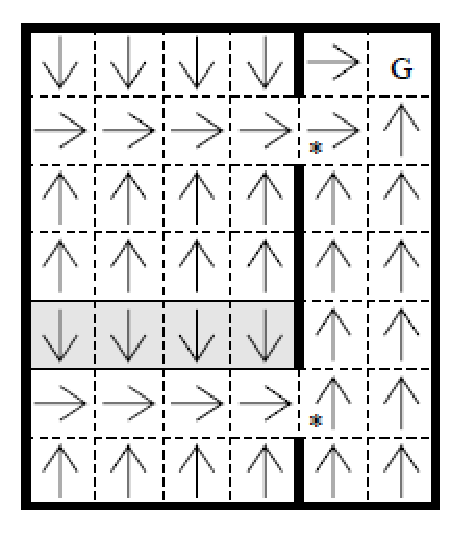
\includegraphics[width=2in] {./figures/Maze.eps}
\end{center}
\caption{A simple maze problem \cite{MaxQJ}.}
\label{fig:Maze}
\end{figure}
\begin{figure}[t]
\begin{center}
    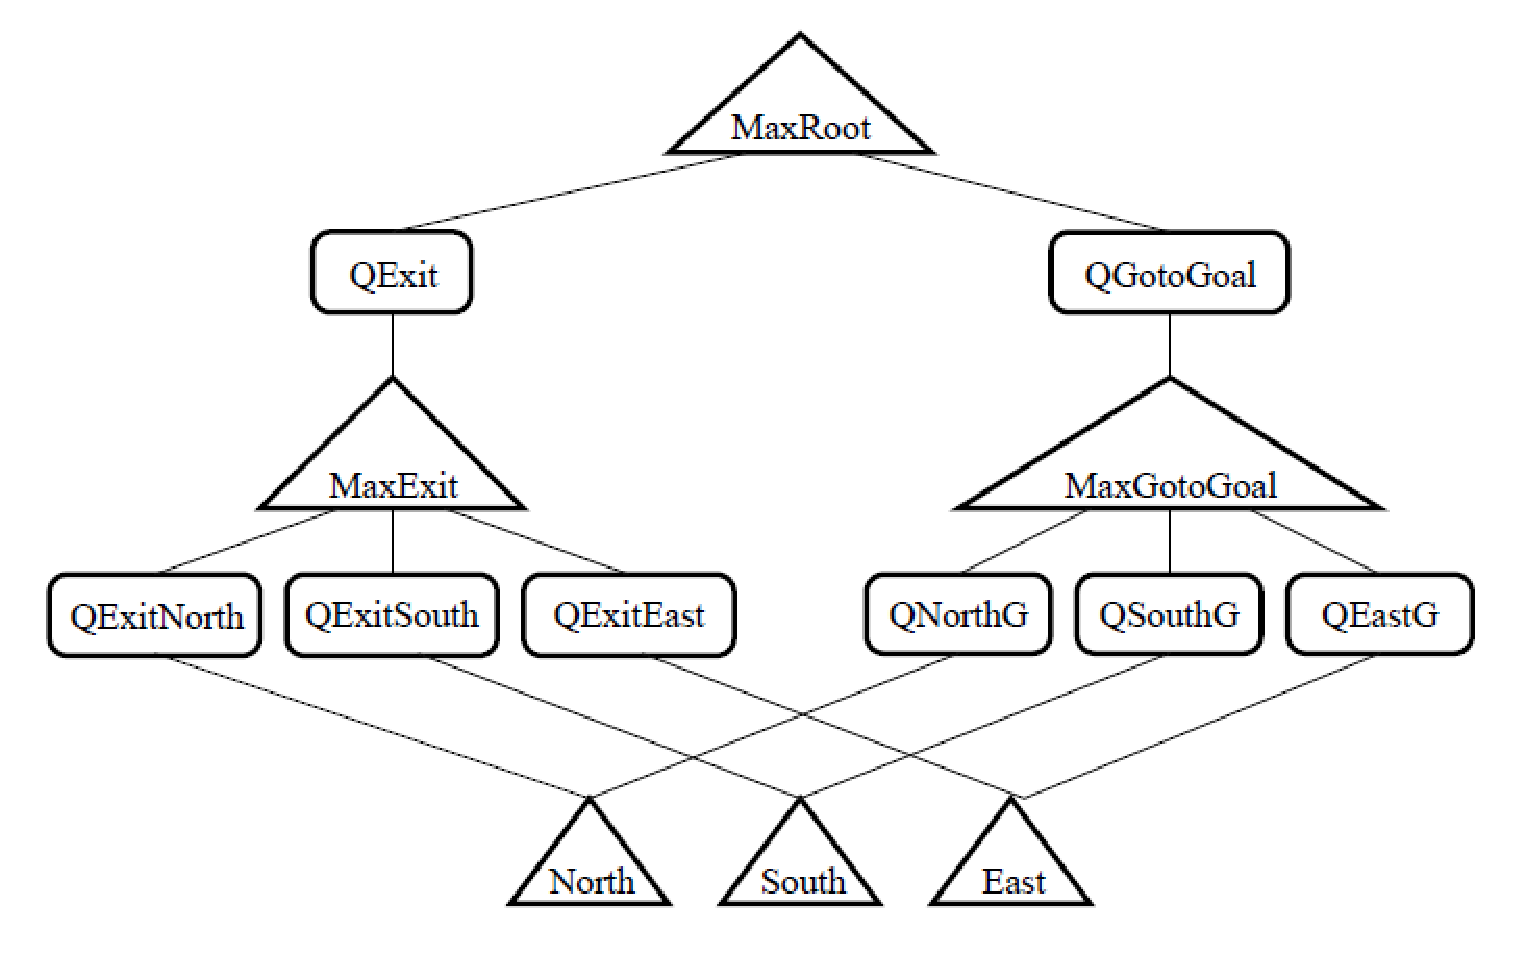
\includegraphics[width=4in] {./figures/MazeH.eps}
\end{center}
\caption{The task hierarchy of the simple maze problem.}
\label{fig:MazeH}
\end{figure}

There are three definitions of optimality of hierarchical reinforcement learning:

\begin{definition}
    \textbf{Optimality:} An optimal policy $\pi^*$ for MDP $M$ is a policy that achieves the highest cumulative reward
    among all policies for the MDP.
\end{definition}
\begin{definition}
    \textbf{Recursive Optimality:} A recursively optimal policy for MDP $M$ with hierarchical 
    decomposition $M' = \{M_0, M_1, \dots, M_n\}$ is a policy $\pi = \{\pi_0, \pi_1, \dots, \pi_n\}$ such
    that each policy $\pi_i$ achieves the highest cumulative pseudo-reward for the corresponding subtask $M_i$,
    assuming fixed policies for its action $A_i$, 
\end{definition}
\begin{definition}
    \textbf{Hierarchical Optimality:} Given $Pi_H$, which is the set of all policies consistent with hierarchy $H$, 
    then a hierarchically optimal policy for MDP $M$ is a policy $\pi^* \in Pi_H$ that achieves the highest cumulative reward
    among all policies $\pi \in Pi_H$.
\end{definition}

An optimal policy is what we want to find for any MDP $M$. However, it may not be possible to 
be found due to the constraints imposed by the hierarchy. Instead of seeking optimality, 
we can seek hierarchical optimality or recursive optimality, which are two important 
optimality guarantee in hierarchical reinforcement learning.

Recursive optimality guarantees that the policy of each subtask is optimal given the policies of its child subtasks.
In this form of optimality, each subtask learns the optimal policy while ignoring the policy from its ancestors
and the all subsequent rewards after the agent arrives the terminal states of the subtask.
Recursive optimality allows the policy of subtask to be reused for different hierarchies. Since
each subtask only needs to seek the optimality within its own subproblem, it is also possible
to adopt state abstraction by ignoring the state variables which are irrelevant
to the subproblem. The MAXQ-Q \cite{MaxQJ} algorithm converges to a recursively optimal policy. 

A hierarchically optimal policy is the policy which achieves the highest cumulative reward given the
hierarchical constraints. The hierarchically optimal policy is a stronger form of optimality. It
may achieve a higher cumulative reward than a recursively optimal policy. In hierarchical optimality, 
the policy of each subtask may not be optimal within its own subproblem, but the overall policy 
of the entire hierarchy is optimal. The HAMQ \cite{HAMQ}, SDMP \cite{SMDP}, tracked Q and HORDQ \cite{HORDQ} algorithms learn
a hierarchically optimal policy.

%TODO: pros and cons for HO and RO
Dietterich \cite{MaxQJ} demonstrates the difference of recursively and hierarchically optimal policies 
with a simple Maze problem (Fig. \ref{fig:Maze}). A robot starts at left room and it needs to reach 
the goal $G$ in the right room. It has three primitive actions, North, South and East.  
The robot receives a reward of -1 for each move.
There are two subtasks, Exit and GotoGoal. Subtask Exit terminates when the robot exits the left room,
and GotoGoal terminates when the robot reaches the goal. The arrows in Figure \ref{fig:Maze} show the 
recursively optimal policy. The arrows in the left room indicate a policy which seeks to exit
the left room with minimum steps. The arrows in the right room seek a shortest path to the goal.
Note that the policy in the shaded area is a recursively optimal but not hierarchically optimal and also not
optimal. A hierarchically optimal policy should exit the left room by the upper door, but a recursively 
optimal policy always exits the room with minimum moves since
a recursively optimal policy ignores the consequences after the subgoal is achieved. 

%TODO: why do we need HO to do the optimal planning
Despite the fact that a hierarchically optimal policy is better than a recursively optimal policy, 
the algorithms which learn the hierarchically optimal policy do not always yield a speedup over
the flat algorithms such as Q-learning or SARSA \cite{MaxQJ, Andre02}. 

\subsubsection{Value Function Decomposition}

Let state $s = (x, y)$, where $x$ consists of planning variables and $y$ consists of environment
variables. Following the MAXQ approach, we decompose the Q-function as:
\begin{equation}
    Q^{\pi}(i, x, j) = Q_r^{\pi}(i, x, j) + Q_c^{\pi}(i, x, j),
    \label{eq:biasedMaxQ}
\end{equation}
where $Q_r^{\pi}(i, x, j)$ is provided by the child subtask $M_j$.

The task of subtask $M_i$ is to compute $Q_c^{\pi}(i, x, j)$ by:
\begin{equation}
    Q_c^{\pi}(i, x, j) = \sum_{x'} P_m^{\pi}(x'|s, j)[Q_r^{\pi}(i, x', \pi_i(x')) + Q_c^{\pi}(i, x', \pi(x'))],
    \label{eq:biasedQc}
\end{equation}

With the formula above, the Q-values can be computed by dynamic programming.

For simplicity, we use the multi-time model \cite{SMDP} to model the transition function: 
\begin{equation}
    P_m(x|s, j) = \sum^{\infty}_{N=1} \gamma^N P(x, N|s, j).
    \label{eq:multiProb}
\end{equation}

$P_m(x|s, j)$ can be estimated by:
\begin{equation}
    \tilde{P}_m(x|s, j) = (1-\alpha)\tilde{P}_m(x|s, j) + \alpha [ \gamma^N \delta_{x'x}],
    \label{eq:approxP}
\end{equation}
for all $x \in S_i$, where $\delta_{x'x}=1$ if $x' = x$ and is 0 otherwise.

Andre and Russell \cite{Andre02, HORDQ} introduced hierarchical optimal recursive decomposed Bellman equations
which extend the decomposition of MAXQ in a way that hierarchical optimality
can be guaranteed.

The Q-value is decomposed as:
\begin{align}
    \label{eq:HordQ}
    Q^{\pi}(i, s, a) = E[\sum_{t=0}^{\infty}\gamma^t r_t] &= E[\sum_{t=0}^{N_1 - 1}\gamma^t r_t] + E[\sum_{t=N_1}^{N_2 - 1}\gamma^t r_t] + E[\sum_{t=N_2}^{\infty}\gamma^t r_t]\\
                    &= Q_r^{\pi}(i, s, a) + Q_c^{\pi}(i, s, a) + Q_e^{\pi}(i, s, a),
\end{align}
where $r_t$ is the random variable of the reward that the agent receives at step $t$, $N_1$ is the number of primitive actions to finish action $a$, 
and $N_2$ is the number of primitive actions 
to finish subtask $M_i$. $ Q_r^{\pi}$ is the expected cumulative reward for executing action $a$.
$Q_c^{\pi}$ is the expected cumulative reward when subtask $M_i$ finishes after the execution of action $a$. 
$Q_e^{\pi}$ is the expected cumulative reward when the episode ends after the execution of subtask $M_i$ .

%TODO: $Q_r$ 

%Our objective is to prove that we can learn the optimal policy if we use HORDQ \cite{HORDQ} on the subtasks which 
%belong to a total leaf cover.

%The node queries its children node to get the value of $V^{\pi}(a, s)$.
$Q_r^{\pi}$ can be computed as:
\begin{equation}
    Q_r^{\pi}(i, s, a) = 
    \left\{\begin{array}{ll}
        Q_r^{\pi}(a, s, \pi_a(s)) + Q_c^{\pi}(a, s, \pi_a(s))& \mbox{if $a$ is composite} \\
        \Sigma_{s'} P(s'|s, a)R(s'|s, a) & \mbox{if $a$ is primitive} \\  
    \end{array} \right.
    \label{eq:Qr}
\end{equation}
%In our example, to compute $Q^{\pi}(MaxRoot, s, GotoExit)$, "MaxRoot" node would query 
%"MaxExit" node to get $V^{\pi}(GotoExit, s)$.

$Q_c^{\pi}$ can be computed as:
\begin{equation}
    Q_c^{\pi}(i, s, a) = \sum_{s', N} P_{S_i}^{\pi}(i, s', N|s, a)\gamma^N[Q_r^{\pi}(i, s', \pi_i(s')) + Q_c^{\pi}(i, s', \pi(s'))],
    \label{eq:Qc}
\end{equation}
where $P_{S_i}^{\pi}(i, s', N|s, a)$ is the probability that $s'$ is the first state in $S_i$ which
is encountered after the execution of action $a$ which takes exactly $N$ steps to finish. 

%Note that $P(s'|s, \pi(s))$ and $V^{\pi}(a, s)$ are provided by the child Max nodes.
And $Q_e^{\pi}$:
\begin{equation}
    Q_e^{\pi}(i, s, a) = \sum_{s', N} P_{T_i}^{\pi}(k, s', N|s, a)\gamma^N[Q^{\pi}(k, s', \pi_k(s'))],
    \label{eq:Qe}
\end{equation}
where $k$ is the index of parent subtask which invoked subtask $M_i$.

To guarantee the optimality, we cannot use the Q-value of parent subtask $M_k$ to update $Q_e^{\pi}$ of subtask $M_i$ because the 
Q-value might not be correct due to the biased model.  Instead, 
we update $Q_e^{\pi}$ with the Q-value of next subtask in $TC(H)$.
Hence, we modify equation \ref{eq:Qe} as:

\begin{equation}
    Q_e^{\pi}(i, s, a) = \sum_{s', N} P_{T_i}(i', s', N|s, a)\gamma^N[Q^{\pi}(i', s', \pi_{i'}(s')],
    \label{eq:OptQe}
\end{equation}
%\subsection{Taxi Domain}
%%Logic of Adaptive Behavior ->Options, SMDP, MAXQ, HORDQ, HAMQ
%MAXQ. The MAXQ algorithm (Dietterich, 1998, 2000b,a) can be seen as an extension
%of the HSMQ algorithm. It relies on the theory of SMDPs but unlike e.g. the options
%framework, it does not rely on reducing the complete problem to a single SMDP. Instead a
%hierarchical task decomposition in behaviors is assumed to be given, and learning proceeds
%in a way similar to SMDP- or HSMQ-learning. MAXQ learns policies equivalent to HSMQ,
%but in addition, it uses a sophisticated value function decomposition to learn these more
%134
%3.8 ABSTRACTION TYPE V: Hierarchical and Temporal Abstraction
%efficiently. The value of a behavior in the context of its calling parent behavior can be
%decomposed into i) the reward expected while executing it and ii) the discounted reward
%of continuing to execute the parent task after it terminates. Let P be the parent behavior
%of B, then
%QP(s; B) = IP(s; B) + CP(P; s; B)
%where IP(s; B) is the expected total discounted reward that is received while executing
%behavior B from initial state s and CP(P; s; B) is the expected total reward of continuing to
%execute behavior P after B has terminated, discounted appropriately with respect to the
%time spent on executing behavior B.
%Pickup
%North East
%t/source
%Put
%Putdown
%South West
%Get
%t/destination
%Root
%Navigate(t)
%Figure 3.18: An example of hierarchical abstraction:
%the MAXQ task hierarchy (Dietterich,
%2000a). The hierarchy constrains the policy space
%in the taxi domain. The leaves of the tree contain
%basic actions in the domain (such as North) and
%the inner nodes represent behaviors that are constructed
%using actions and behaviors lower in the
%tree. Note that the Navigate behavior is reused
%for both getting to the passenger and delivering
%him, and also that it is parameterized using the
%target location.
%The IP(s; B) can be recursively decomposed
%into I and C following
%IP(s; B) = max
%a2AB
%QP(s; a)
%There are several advantages of this decomposition,
%specifically in learning recursively
%optimal Q-values. Both the I and C functions
%can be represented using different state
%space abstractions, allowing for sharing (and
%compactness) in the representation of the
%value function. See (Dietterich, 2000a) for
%more subtle details on this decomposition.
%HAMQ. Q-learning with hierarchies of abstract
%machines (HAMQ) (Parr and Russell,
%1998) learns hierarchically optimal policies,
%and uses devices resembling finite-state machines
%to implement behaviors. These machines
%include an internal state and this state
%determines the actions that are taken. Like
%the options framework, HAMs are based on
%the SMDP model, though the aim here is not
%to enlarge the action space with behaviors, but instead to simplify large MDPs by restricting
%the policy space. The core idea in HAM is that the policies for the original MDP are
%defined as programs which execute based on their own state as well as the state of the
%underlying MDP. There are several types of actions. There are primitive actions, actions
%that terminate the current behavior and return control to the calling behavior and actions
%that call other behaviors. Learning takes place only at choice points where a behavior
%must decide which of several internal transitions to make. These choice-points represent
%a trade-off between fully hard-coded policies and learned policies. All the finite state machines
%representing the behaviors are compiled into one machine where the learning takes
%place. Andre and Russell (2001) extended the framework to programmable HAMs, adding
%interrupts and the ability to pass parameters, among other things, and later extended the
%programming language to ALISP (Andre and Russell, 2002, see also Chapter 7).



